\section{Analyse}
\subsection*{H�jttalerens impulsrespons}
Af figur \ref{impuls} ses, at impulsresponset er forholdsvist kort, ca. 5 ms, hvilket natuligvis stemmer overens med, at responset er optaget i et lydd�dt rum.

\subsection*{Frekvenskarakteristikken generelt}
I figur \ref{all} er alle m�lingerne vist samlet med og uden NXT-kabinettet p�sat. Generelt fremg�r det, at h�jttaleren ikke siger meget under 600 Hz, hvilket naturligvis h�nger sammen med h�jttalerens diameter p� ca. 30 mm. Derudover observeres en line�r frekvensgang set i forhold til at det er en lille h�jttaler.

\subsection*{Spredningskarakteristik og kabinettets p�virkning}
I figur \ref{orto}, sammenholdes m�linger med vinkler mellem $-40\,^{\circ}$ og $0\,^{\circ}$ horisontalt og vertikalt. Dette illustrerer h�jttalerens spredningskarakteristik, og det fremg�r at vinklen ikke betyder det store for frekvensspektret.

Der er dog generelt st�rre spredning p� m�lingerne ved den horisontale vinkel�ndring, hvilket kan skyldes p�virkning fra kabinettets vertikale riller, se figur \ref{kabinet}.

\begin{figure}[h!]
\begin{center}
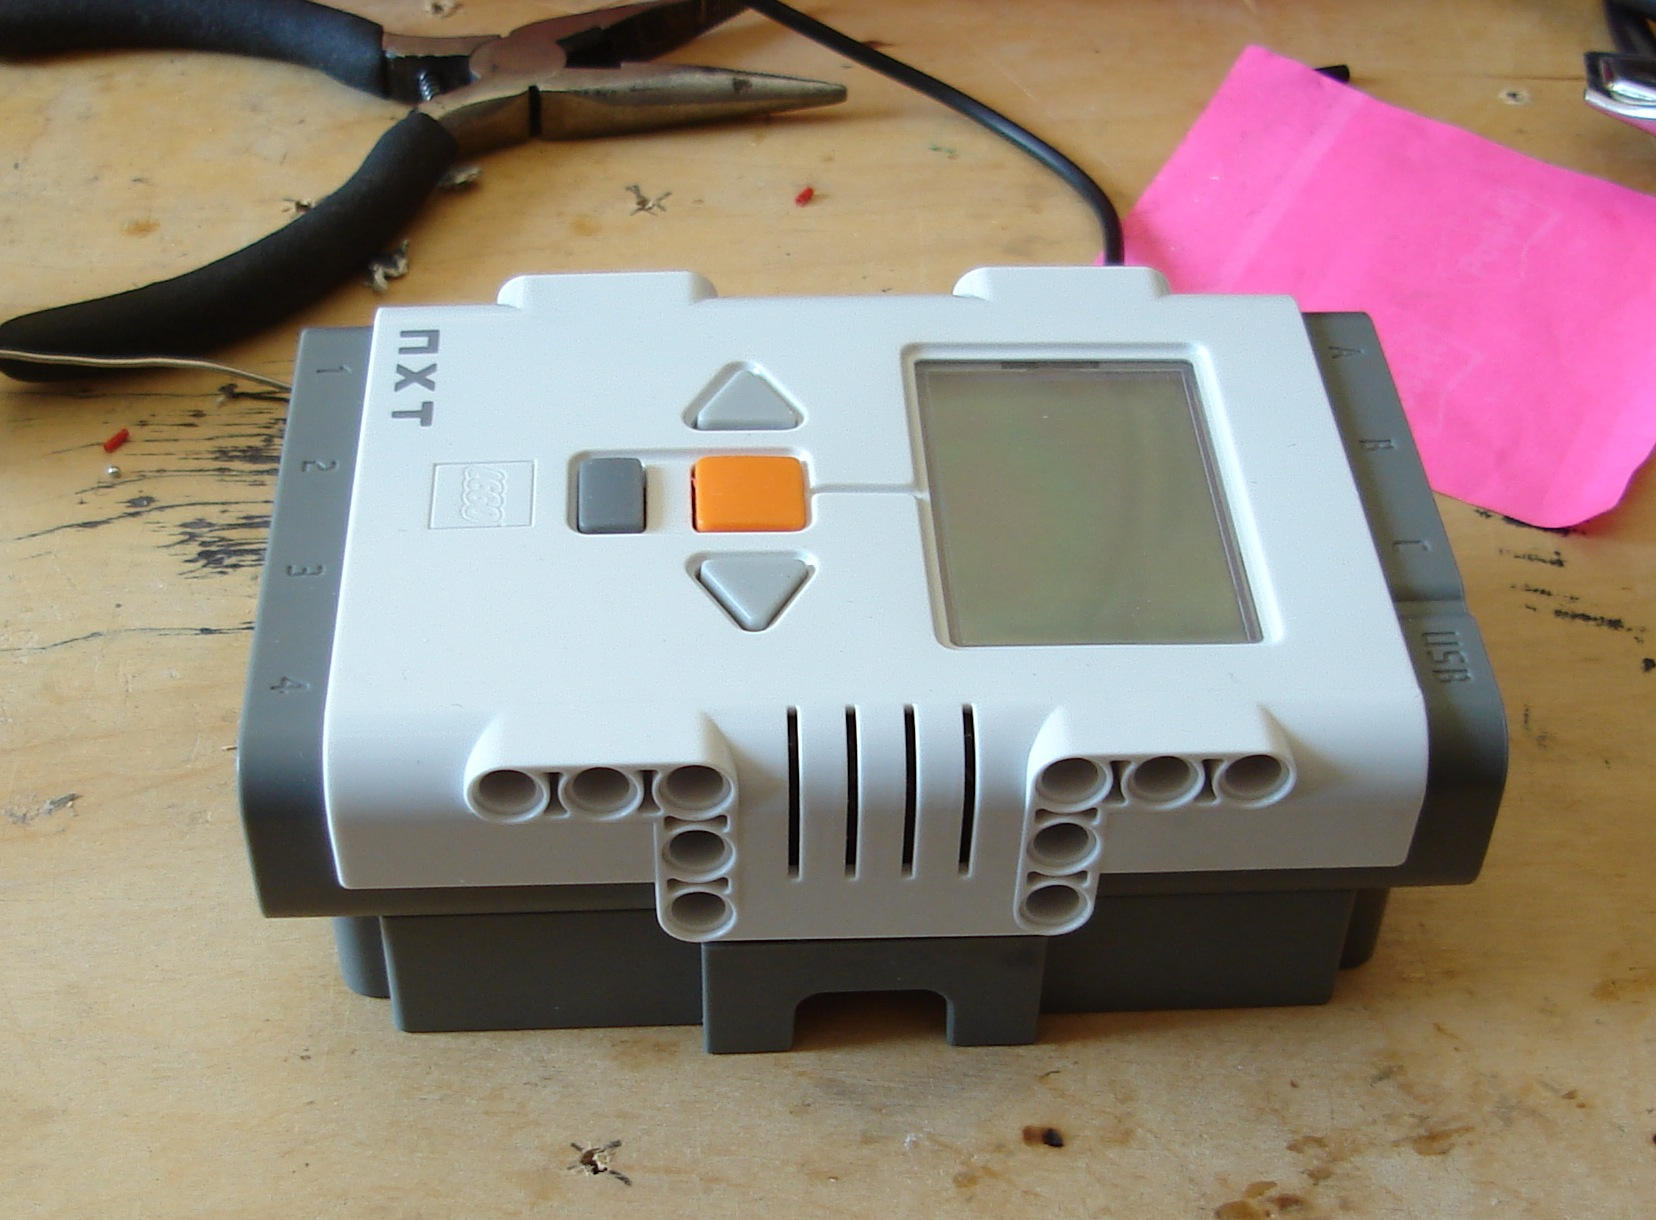
\includegraphics[width=8cm]{kabinet.jpg}
\end{center}
\caption{NXT'ens kabinet med de vertikale riller}
\label{kabinet}
\end{figure}

I figur \ref{onaxis} sammenlignes on-axis m�linger for h�jttaleren med og uden NXT-kabinettet p�sat. Det ses at kabinettet giver en betydelig p�virkning ved godt 2 kHz med et dyk p� ca. 10 dB. 

